%% 
%% Copyright 2019-2024 Elsevier Ltd
%% 
%% Version 2.4
%% 
%% This file is part of the 'CAS Bundle'.
%% --------------------------------------
%% 
%% It may be distributed under the conditions of the LaTeX Project Public
%% License, either version 1.2 of this license or (at your option) any
%% later version.  The latest version of this license is in
%%    http://www.latex-project.org/lppl.txt
%% and version 1.2 or later is part of all distributions of LaTeX
%% version 1999/12/01 or later.
%% 
%% The list of all files belonging to the 'CAS Bundle' is
%% given in the file `manifest.txt'.
%% 
%% Template article for cas-sc documentclass for 
%% single column output.

\documentclass[a4paper,fleqn]{cas-sc}

\usepackage[numbers]{natbib}

% Additional packages
\usepackage{amsmath,amssymb,amsfonts}
\usepackage{algorithmic}
\usepackage{textcomp}
\usepackage{xcolor}
\usepackage{booktabs}
\usepackage{array}
\usepackage{microtype}
\usepackage{tikz}
\usetikzlibrary{arrows.meta, shapes.geometric, positioning}
\usepackage{float}
\usepackage{placeins}

%%%Author definitions
\def\tsc#1{\csdef{#1}{\textsc{\lowercase{#1}}\xspace}}
\tsc{WGM}
\tsc{QE}
\tsc{EP}
\tsc{PMS}
\tsc{BEC}
\tsc{DE}
%%%

\graphicspath{{./}{./images/}}

\begin{document}
\let\WriteBookmarks\relax
\def\floatpagepagefraction{1}
\def\textpagefraction{.001}
\shorttitle{Edge-based Fossil Species Classification}
\shortauthors{A. Gupta et al.}

\title [mode = title]{Edge-based (Mobile) Fossil Species Classification using MobileNetV2}                      

\author[1]{Dr. Anshu Gupta}
\cormark[1]
\ead{aagupta@kkwagh.edu.in}

\credit{Conceptualization of this study, Methodology, Supervision, Project administration}

\affiliation[1]{organization={Department of Electronics and Telecommunication, K.K. Wagh Institute of Engineering Education and Research},
                city={Nashik},
                state={Maharashtra},
                country={India}}

\author[1]{Anurag Mohod}
\ead{asmohod370223@kkwagh.edu.in}

\credit{Data curation, Software implementation, Writing - Original draft preparation, Validation}

\author[1]{Ishaan Narakesari}
\ead{ianarakesari370223@kkwagh.edu.in}

\credit{Investigation, Formal analysis, Visualization}

\cortext[cor1]{Corresponding author}

\begin{abstract}
For the purpose of scientific documentation and understanding evolutionary history of that species, accurately identifying fossil species is vital in paleontology. This process faces some challenges that are yet to be addressed. Fossil excavations in remote areas with no network can be challenging and analysis might be delayed till later in labs or heavier computational setups might be needed. This paper aims to address these challenges and proposes a simulation--based solution. We propose a mobile (edge) based fossil species classification system that is trained on dataset containing the images of Radiolarian species fossils and a lightweight convolutional neural network deployed on the mobile. This solution enables fossil classification in remote areas and preliminary analysis is performed immediately on--site. We evaluated the model on metrics like F1 score, precision, recall. The model attains 91.8\% accuracy. This approach enables early classification of fossil specimens.
\end{abstract}

\begin{highlights}
\item Mobile-based fossil classification enabling on-site analysis in remote areas without network connectivity
\item MobileNetV2 architecture achieving 91.8\% accuracy on Radiolarian microfossil dataset
\item Int8 quantized model outperforming float32 baseline with improved efficiency for edge deployment
\end{highlights}

\begin{keywords}
TinyML \sep paleontology \sep CNN \sep MobileNetV2 \sep edge computing \sep radiolarian microfossils
\end{keywords}

\maketitle

\section{Introduction}

Fossil classification plays an important part in the documentation of fossils and the study of phylogenetic histories. The morphological characteristics of fossils offer vital information in the development of phylogenetic lineages. Technology has greatly improved the classification of fossils, especially through modern computers' powerful computer algorithms~\cite{hsiang2019machine,sun2023deep}. However, there are a number of hurdles or setbacks. In areas without internet access as a result of geographical factors, the classification of fossils occurs slowly or is put on hold. Extensive logistical challenges are responsible for the difficulties experienced in areas with poor electrical power and internet access. This has created a major bottleneck between fossil classification and decision-making. Prior work has not solved these challenges yet, as existing machine learning solutions predominantly rely on cloud-based inference or workstation-grade hardware, neither of which is feasible in the context of expedition-based paleontology. This paper aims to propose a simulation--based solution to address the gaps mentioned. A mobile--based fossil classification solution that uses a lightweight CNN, deployed locally on mobile devices is proposed. The MobileNetV2~\cite{sandler2018mobilenetv2} model is used to be pretrained on the Radiolarian dataset, in order to perform fossil classification for the preliminary analysis. The architectural design of MobileNetV2, with its inverted residual structure and linear bottleneck layers~\cite{sandler2018mobilenetv2}, provides a favorable balance between representational capacity and computational efficiency, rendering it suitable for deployment on resource-constrained mobile processors. We evaluated the model on the F1 score, precision and recall metrics as well as made the confusion matrix. The model showed 91.8\% accuracy. Although no comparable work exists, the accuracy highlights the viability of our solution. This performance level is particularly noteworthy given the morphological complexity inherent in radiolarian skeletal structures and the relatively limited size of annotated training data available for this taxonomic group. This solution ensures early real time fossil classification on--site and can aid the paleontologists for the same.

Often, field paleontology requires timely decision-making on fossil samples collected from remote environments where connectivity and computational power are limited. This often prompts difficulties resulting from the current standard process of using lab-based or cloud-based inference. A disconnect between sample collection and species identification creates a dilemma because timely decision-making for adaptability is limited. This problem can effectively be solved by using classification systems. In this regard, radiolarian microfossils are of great scientific value because of their global distribution, high rates of evolution, and susceptibility to past oceanographic conditions~\cite{brombacher2020radiolarian}. As marine protozoans, these extremely diverse microfossils have siliceous skeletons that have been constantly evolving since the Cambrian era~\cite{brombacher2020radiolarian}. In addition, these microorganisms are found everywhere in the oceans and are useful in dating geological samples because of their short stratigraphic range of about 1-3 million years~\cite{brombacher2020radiolarian}.

The siliceous skeletons of radiolarian microfossils have complex morphologies that provide critical diagnostic information for species classification, but at the same time, they are difficult to interpret using computational models. The three-dimensional lattice structures of these skeletons, characterized by radial symmetry, pore variability, and species-specific ornamentation, add to the difficulty of computer-assisted pattern recognition. These structures have to be deduced from two-dimensional microscopy images, which by their nature lack depth information and can vary due to factors such as sample orientation, preservation quality, and imaging conditions. The scarcity of trained micropaleontologists, combined with the labor-intensive nature of manual identification (often requiring hours per sample), creates a bottleneck in paleoceanographic research and limits the throughput of biostratigraphic analysis in industrial and academic contexts.

The current research attempts to overcome the challenge by proposing a lightweight convolutional neural network for the identification and detection of microfossils within disconnected settings. Inspired by previous works for edge deployment in fossil classification~\cite{lin2022edge}, the proposed approach permits the direct recognition and detection of fossils within their native habitat. Unlike other approaches, it combines classification and detection within a single deployable model, avoiding end-to-end processing chains and associated cumulative delays for detection and classification. This research is not optimized for the best possible results in a disconnected environment but tackles the problem of how geologists carry out their work in the field. The primary design constraint is operational feasibility rather than maximum achievable accuracy, reflecting the practical reality that a moderately accurate system available immediately at the point of collection is more valuable for field decision-making than a highly accurate system requiring delayed laboratory analysis.

\FloatBarrier

\section{Installation}

This paper proposes a mobile-based fossil classification system that scans a fossil using the camera and classifies the species. The open-source nature of the dataset promotes the idea of verifiability of the results of the research, which is in line with the current paradigms that regulate the use of machine learning in scientific research.

The dataset used in this research is a set of high-resolution microscopy images of individual radiolarian specimens. The choice of radiolarian specimens is based on their importance. The fact that they are abundant in marine plankton and consist of protozoans with silica shells makes them extremely valuable for biostratigraphic and paleoenvironmental research~\cite{brombacher2020radiolarian}. The high-quality preservation of their fossil skeletons, which is due to the chemical stability of their skeletons during diagenesis, provides a vast fossil record over the Phanerozoic.

The taxonomic diversity of Radiolaria, which is supported by more than 10,000 known species with unique morphological features~\cite{brombacher2020radiolarian}, provides a solid foundation for the investigation of the ability of convolutional feature detectors to distinguish between species. However, the varying preservation of the structures in the sediment samples results in a limited annotated micro-image dataset for the current study. Taphonomic factors affecting the micro-organisms, which include dissolution, fragmentation, and distortion, contribute considerable intra-species variability, requiring the incorporation of these factors in the training dataset for better generalization performance. This problem of micro-image classification attempts to assess the discriminative ability of convolutional neural networks for Radiolaria, based on the complexity of their morphology. The characteristic lattice patterns of Radiolaria, combined with micro-level structural details, provide a rich data set to assess the ability of convolutional neural networks to identify sufficiently discriminative information to enable accurate classification.

Radiolaria are unicellular eukaryotes that range in diameter from 0.1 to 0.2 mm and have complex siliceous skeletons with radial symmetry. The general skeletal pattern consists of a series of concentric shells that are joined by radial spines, although the number of shells, distribution of pores, and shape of spines differ among species and often provide the first means of diagnosis.

Images are described as two-dimensional matrices (height by width) with a single intensity channel. Grayscale image representation is valid, as transmitted-light microscopy of siliceous microfossils produces images that are nearly achromatic, with contrast provided by differences in optical density rather than chromatic absorption. This simplification eliminates redundant chromatic information while retaining diagnostic morphological intensity information, which reduces computational complexity with little loss of diagnostic resolution. Post-training quantization to int8 precision reduces model size by approximately 75\%, with calibration on representative training data maintaining numerical stability and keeping quantization error within acceptable limits for classification~\cite{edgeimpulse2023}. Quantization-aware deployment leverages evidence indicating that reduced-precision inference maintains or improves generalization while significantly reducing latency and energy consumption in embedded systems~\cite{yaqoob2024tinyml}. The regularizing impact of the quantized noise is again an extensively validated effect in all domains that prevents model complexity through precision limitations, thereby avoiding overfitting to data idiosyncrasies~\cite{yaqoob2024tinyml}. For fossil classification, with annotated examples in short supply and well-preserved examples even scarcer, regularization is very beneficial. Finally, utilization of int8 operations can leverage hardware acceleration through mobile NPUs and ARM NEON instructions to produce substantial throughput and energy savings.

\FloatBarrier

\section{Front matter}

Source of Dataset: Annotated radiolarian microfossil image set sourced through the Edge Impulse pipeline. The original source of the radiolarian image dataset used lies at Zenodo (DOI:10.5281/zenodo.6565553). This was originally uploaded on May 20, 2022. All images are licensed under the Creative Commons Attribution 4.0 International License. This grants permission for redistribution and reuse of these images with proper attribution. The open-source nature of our dataset improves the verifiability of research results, which corresponds with modern paradigms that promote the use of machine learning in scientific fields.

For our research, we use a set of high-resolution microscopy images of individual radiolarian specimens. Radiolaria were selected for their importance: their abundance in marine plankton and their silica-cased protozoan biology make them extremely useful for biostratigraphic and paleoenvironmental studies~\cite{brombacher2020radiolarian}. Skeletal preservation of the Radiolaria is quite good due to the chemical stability of these organisms. With more than 10,000 species of well-known variability based on the possession of different morphological characteristics~\cite{brombacher2020radiolarian}, the substantial taxonomy of Radiolaria forms a comprehensive platform upon which the capability of convolutional feature detector models to distinguish between different species may be assessed. However, the observability of skeleton patterns exhibits variability with limited possibilities for the availability of an annotated image set. Taphonomic variability such as dissolution, fragmentation, and distortion is quite significant.
Here, the micro image classification problem focuses specifically on the discriminative potential of Convolutional Neural Networks (CNN) in the context of Radiolaria, along with their intricate structures. The lattice-like features of Radiolaria micro-structure arising from their skeletons are suitable for evaluating the discriminative potential of CNN in extracting relevant features for precise image classification. Radiolaria, being unicellular eukaryotes measuring 0.1-0.2 mm in diameter, bear complex siliceous skeletons showing radial symmetry. Their typical arrangement comprises multiple shells and their connecting radial spines, which may differ across species in the number of shells and arrangement of the pores and spine structure.
Images are modeled as two-dimensional matrices with a fixed height, width, and a single intensity channel. Grayscaling is suited for transmitted light microscopy of siliceous microfossils, creating nearly achromatic images where contrast is based on optical density rather than chromatic absorption. This process removes redundant chromatic data while retaining necessary intensity-contrast morphological information.

The database consists of high-resolution TIFF images showing various radiolarian morphotypes at various stages of preservation. The TIFF image format preserves all camera-to-sensor data and does not compress images, which could degrade diagnostic morphological structures used to classify radiolarian species. In order to enhance the detectability of sparse specimens and reduce class imbalance, patch-based extraction was performed~\cite{liu2023patch}. Sliding-window approaches on whole-slide images generate numerous training examples per specimen and increase dataset size while preserving biological variation. Deliberate oversampling of rare species is done through targeted patch harvesting to handle class imbalance~\cite{zhang2024class}.
The task was carried out as classification between various classes of radiolarian species and background, and another as an object detection problem where bounding box localization with classification was implemented. By framing it as a dual-task problem, the system not only has the ability to classify different specimens but also has the ability to localize different structures of the radiolarian specimen, especially when there are several sediment particles, fragments of microfossil material, and imaging artifacts present in a field of view.
The data is divided into 85\% for training and 15\% for the test set, which is stratified for the different radiolarian species. Stratified splitting distributes the different species in the test set as well as the training set according to their natural distribution in the overall set. By this splitting, the bias in the test set cannot be immense, which would have occurred if the test set was simply divided into the different species.
After data augmentation, we have finally obtained a last set of data consisting of labeled images of radiolarians, which totals 3,625. The current number is adequate, as it covers a number of diverse biological specimens which can efficiently be prepared with the methods of deep learning~\cite{hsiang2019machine}. Specifically, although this number of images seems small for contemporary computer vision, in the particular field of micropaleontology, a number of datasets does not exceed a few thousand specimens, due to the difficulty in their label creation.
For processing the TIFF image data for classification, the approach was to convert all the TIFF images into a single-channel grayscale image through the use of the average function over the existing channels. This approach ensured that the important morphology of the skeletons in the images of the radiolarians was preserved but in a simpler form with increased invariance to lighting. This was done to effectively perform the noise reduction function of the image data to be processed through the average function calculation over the available channels, which statistically acts to improve the signal-to-noise ratio in the input data to the neural network.
The images were also resized to a uniform size of 96 × 96 pixels, employing a technique of bilinear interpolation. The choice of the resolution, which is 96 × 96 pixels, involves a decision to take into account the optimization of spatial resolution, which is necessary to accommodate diagnostic morphological features, while considering the computational efficiency necessary to enable real-time inference that can be accomplished by mobile processors. The process of bilinear interpolation was used to ensure the images were not made worse by the interpolation, which can result in undesirable aliasing effects. When the resized images were not able to maintain the original aspect ratio, they were also subject to a center crop, which ensured that the radiolarian was centered in the images, thus choosing to maintain the images of the specimen's internal structures, which are typically the most informative, while sacrificing some detail that is not as relevant taxonomically.
Then, intensity values were then normalized by division by 255. This linear scaling maps pixel intensities from their original integer range to the floating-point range expected by the neural network, which helps to stabilize gradient magnitudes during backpropagation and accelerates convergence. Images were center-cropped based on aspect ratio, then resized to 96 × 96 pixels. Normalization of pixel intensity to a standard range for processing was performed next([0,1]). The present standardized pre-processing pipeline ensures that all input samples are consistent, and this avoids any systematic bias in results that might arise due to variability of imaging conditions across different microscopy sessions.

\begin{figure}[htbp]
\centering
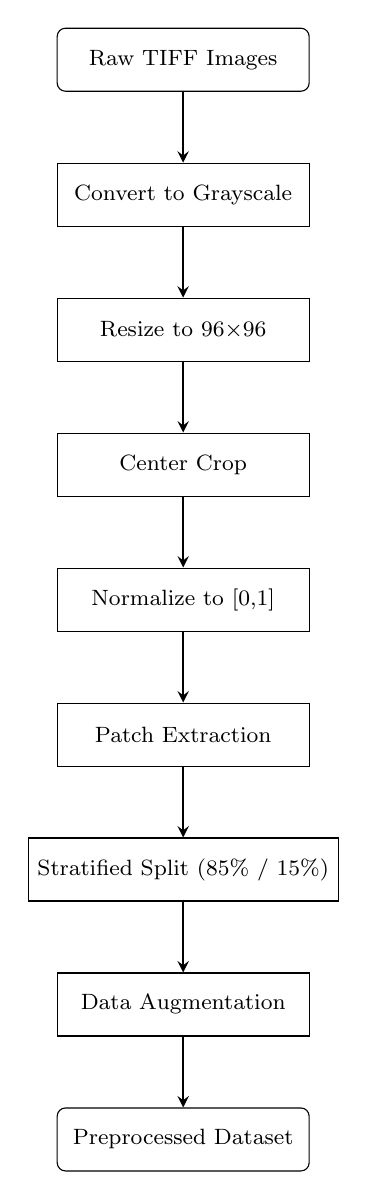
\begin{tikzpicture}[
    node distance=0.9cm,
    every node/.style={font=\footnotesize},
    startstop/.style={
        rectangle, 
        rounded corners=3pt,
        minimum width=3.2cm, 
        minimum height=0.8cm,
        text centered, 
        draw=black
    },
    process/.style={
        rectangle, 
        minimum width=3.2cm, 
        minimum height=0.8cm,
        text centered, 
        draw=black
    },
    arrow/.style={thick, ->, >=stealth}
]

\node (start) [startstop] {Raw TIFF Images};

\node (convert)   [process, below=of start]    {Convert to Grayscale};
\node (resize)    [process, below=of convert]  {Resize to 96$\times$96};
\node (crop)      [process, below=of resize]   {Center Crop};
\node (normalize) [process, below=of crop]     {Normalize to [0,1]};
\node (patch)     [process, below=of normalize]{Patch Extraction};
\node (stratify)  [process, below=of patch]    {Stratified Split (85\% / 15\%)};
\node (augment)   [process, below=of stratify] {Data Augmentation};

\node (end) [startstop, below=of augment] {Preprocessed Dataset};

\draw [arrow] (start) -- (convert);
\draw [arrow] (convert) -- (resize);
\draw [arrow] (resize) -- (crop);
\draw [arrow] (crop) -- (normalize);
\draw [arrow] (normalize) -- (patch);
\draw [arrow] (patch) -- (stratify);
\draw [arrow] (stratify) -- (augment);
\draw [arrow] (augment) -- (end);

\end{tikzpicture}
\caption{Flowchart 1 -- Data Preprocessing and Preparation Pipeline}
\label{fig_preprocessing}
\end{figure}

\begin{figure}[htbp]
\centering
\includegraphics[width=0.5\textwidth]{sample 1 - image.JPG}
\caption{Classification sample 1}
\label{fig_specimen_diversity}
\end{figure}

\begin{figure}[htbp]
\centering
\includegraphics[width=0.5\textwidth]{sample 2 - image.JPG}
\caption{Classification sample 2}
\label{fig_class_distribution}
\end{figure}

\FloatBarrier

\section{Bibliography styles}

MobileNetV2~\cite{sandler2018mobilenetv2} has achieved tremendous traction in the field of mobile and embedded vision applications due to the inverted residuals and linear bottleneck. This makes it more suitable for TinyML~\cite{warden2019tinyml}. The inverted residual module adds dimensionality at intermediate points of the network and not on the boundaries of the residual blocks. This prevents memory bandwidth utilization. Dimensionality reduction on the interfaces of the residual blocks helps keep the tensors low-dimensional throughout the networks. Quantizing the floating-point tensors of the models to the closest integer values results in reduced memory consumption and faster computation with minimal loss of model performance~\cite{edgeimpulse2023}. This procedure of int8 quantization makes the best use of the redundancy involved in the neural network. Is the float to signed integer conversion an acceptable procedure? Calibration is done by computing the scale and offset from representative tensors of the activation values. This procedure makes sure that the quantized network has the exact same functionality as the float network, converging within certain tolerance thresholds.


Several studies demonstrate the effectiveness of convolutional neural networks for microfossil and plankton classification, including radiolarians, foraminifera, pollen, and other microfossils~\cite{keceli2017automated,dionisio2020automated,marchant2020artificial,lin2017focal}. These investigations collectively establish that discriminative features for species-level identification can be learned from microscopy imagery through supervised training of deep networks. The translation invariance and hierarchical feature extraction properties of CNNs align well with the pattern recognition requirements of fossil classification, where diagnostic morphologies appear at multiple spatial scales and variable orientations. More recent work has explored vision transformers and hybrid architectures for fossil imagery, reporting improvements in capturing long-range morphological dependencies but at substantially higher computational cost~\cite{sun2023deep,hou2023vision}. Transformer architectures are known for their performance in dealing with global spatial relationships using self-attention mechanisms~\cite{dosovitskiy2021image}. These are expected to be effective for understanding skeletal configurations within radiolarian image data. However, the quadratic computational cost for computing attention across sequences and the high parameter count mean they are not expected to be deployed on mobile devices under the current technological regime. Large datasets of fossil images and CNN-based classification systems have been set up, which enable statistical studies for different taxa and geographic intervals~\cite{delima2019digital}. Access to comprehensive datasets comprising various taxonomic groups along with appropriate time scales aids in the thorough testing of generalization capability using unseen species and preservation states, beyond conventional measures of single-class classification. However, most reported works have focused on workstation or server-based inference methods, while end-to-end on-device approaches for radiolarian identification are rare, especially when these methods combine classification with object detection within a unified model deployable on devices. This gap between proof-of-concepts in a lab environment and deployable systems in field scenarios acts as a critical hurdle towards the incorporation of machine learning.

\FloatBarrier

\section{Floats}

Here, we utilize MobileNetV2~\cite{sandler2018mobilenetv2}, a light-weight convolutional network especially designed for devices with limited resources like mobile devices, unlike other architectures. At the heart of MobileNetV2 is the widely used depthwise separable convolution operation, which is a spatial and channel separable equivalent to the standard convolution~\cite{sandler2018mobilenetv2}. This reduces computational complexity from \(O(h \times w \times c_{in} \times c_{out} \times k^2)\) to \(O(h \times w \times c_{in} \times k^2 + h \times w \times c_{in} \times c_{out})\), where \(h\) and \(w\) denote spatial dimensions, \(c_{in}\) and \(c_{out}\) represent input and output channels, and \(k\) is the kernel size.
These operations result in lower memory usage and efficiency with performance on mobile devices for our classification model. The lower number of parameters minimizes the storage size of our model for mobile devices, as well as the network bandwidth that will be used to load weights from storage to cache, another important factor for mobile deployment. 
Backbone for this is MobileNetV2, adapted for 96x96 resolution~\cite{sandler2018mobilenetv2}. The adaptation to reduced input resolution requires careful adjustment of stride patterns in early convolutional layers to prevent excessive spatial downsampling that would eliminate fine-grained morphological details before they can be captured by deeper layers.

Compared to existing methods of using heavier computational setups, our solution provides the advantage of early analysis and confirmation of the fossil species on-site itself using no extra hardware apart from the mobile in remote areas with restricted network access. This operational autonomy eliminates dependencies on communication infrastructure and centralized computational resources, enabling paleontological fieldwork in geographically remote locations such as deep-ocean drilling expeditions, polar research stations, and isolated terrestrial formations where connectivity is either unavailable or prohibitively expensive.

\begin{figure}[htbp]
\centering
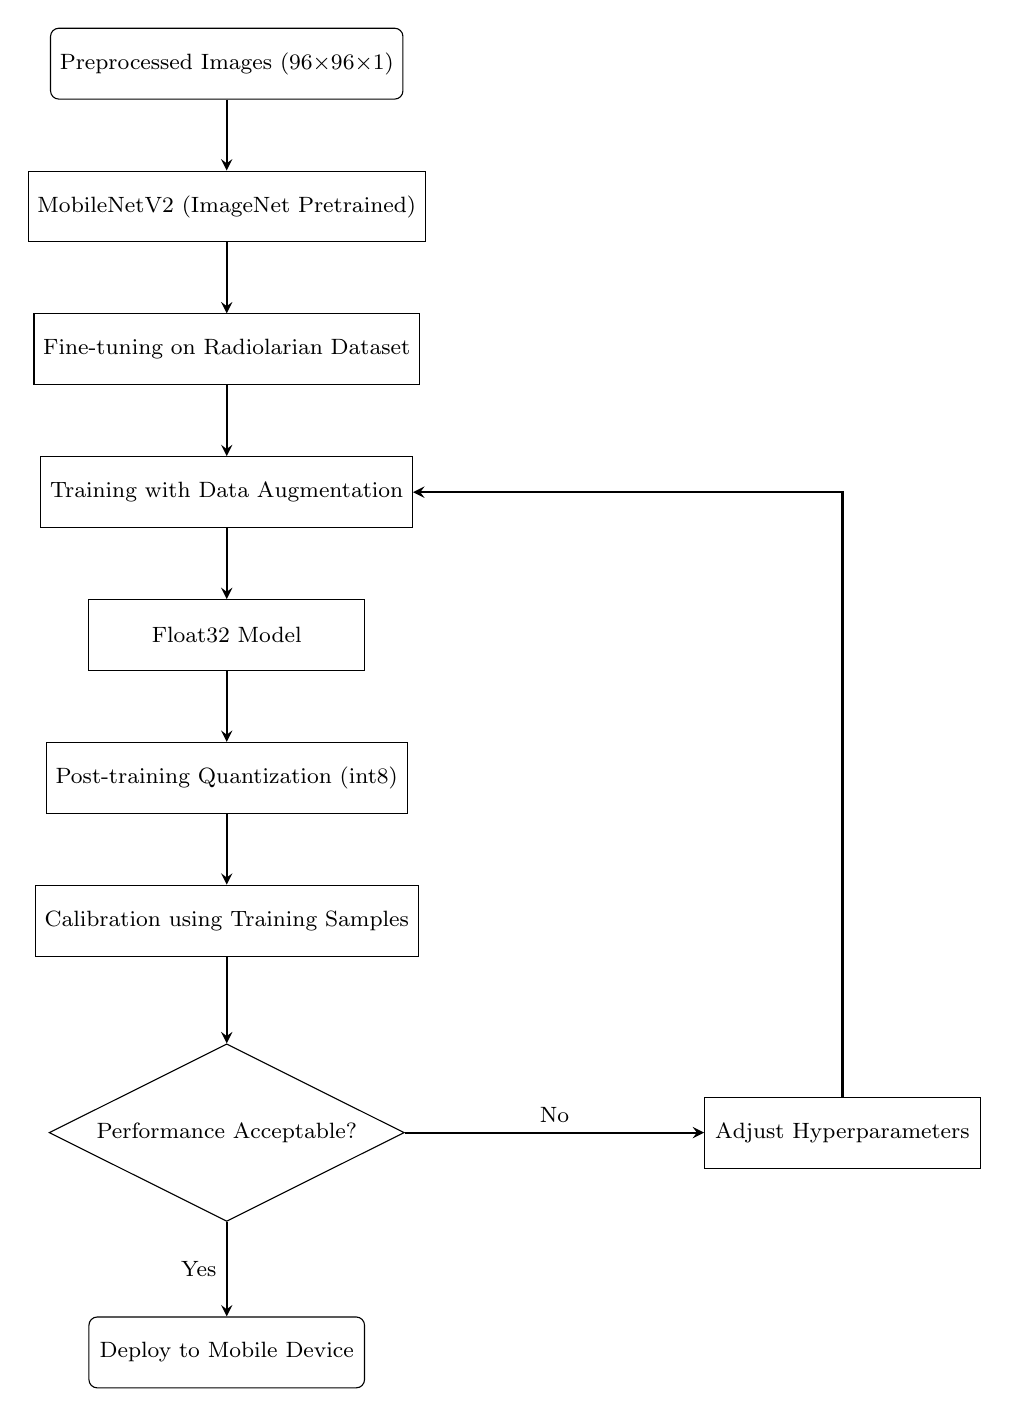
\begin{tikzpicture}[
    node distance=0.9cm,
    every node/.style={font=\footnotesize},
    startstop/.style={
        rectangle,
        rounded corners=3pt,
        minimum width=3.5cm,
        minimum height=0.9cm,
        text centered,
        draw=black
    },
    process/.style={
        rectangle,
        minimum width=3.5cm,
        minimum height=0.9cm,
        text centered,
        draw=black
    },
    decision/.style={
        diamond,
        aspect=2,
        minimum width=3.2cm,
        minimum height=1cm,
        text centered,
        draw=black
    },
    arrow/.style={thick,->,>=stealth}
]

\node (input) [startstop] {Preprocessed Images (96$\times$96$\times$1)};

\node (pretrain)  [process, below=of input]
    {MobileNetV2 (ImageNet Pretrained)};

\node (finetune)  [process, below=of pretrain]
    {Fine-tuning on Radiolarian Dataset};

\node (train)     [process, below=of finetune]
    {Training with Data Augmentation};

\node (float)     [process, below=of train]
    {Float32 Model};

\node (quantize)  [process, below=of float]
    {Post-training Quantization (int8)};

\node (calibrate) [process, below=of quantize]
    {Calibration using Training Samples};

\node (validate)  [decision, below=of calibrate, yshift=-0.2cm]
    {Performance Acceptable?};

\node (deploy) [startstop, below=of validate, yshift=-0.3cm]
    {Deploy to Mobile Device};

\node (retrain) [process, right=3.8cm of validate]
    {Adjust Hyperparameters};

% Arrows
\draw[arrow] (input) -- (pretrain);
\draw[arrow] (pretrain) -- (finetune);
\draw[arrow] (finetune) -- (train);
\draw[arrow] (train) -- (float);
\draw[arrow] (float) -- (quantize);
\draw[arrow] (quantize) -- (calibrate);
\draw[arrow] (calibrate) -- (validate);

\draw[arrow] (validate) -- node[left] {Yes} (deploy);
\draw[arrow] (validate) -- node[above] {No} (retrain);
\draw[arrow] (retrain) |- (train);

\end{tikzpicture}
\caption{Flowchart 2 -- MobileNetV2 Training and Quantization Workflow}
\label{fig_training_workflow}
\end{figure}

\begin{figure}[htbp]
\centering
\includegraphics[width=.5\textwidth]{float32 - 2.JPG}
\caption{Shows the scatterplot of detection outputs of the float32 model. While the green points represent correct classification for the objects, the misclassified points are represented in red. Clearly, the areas containing high percentages of green points indicate high accuracy, whereas the areas containing high percentages of red points indicate failure to detect the data points, providing us with crucial information for further enhancement.}
\label{FIG_1}
\end{figure}

\begin{figure}[htbp]
\centering
\includegraphics[width=.5\textwidth]{int8 - 2.JPG}
\caption{Shows the results from the int8 model for comparison. The quantized model demonstrates comparable spatial distribution of correct and incorrect predictions, indicating that reduced numerical precision does not introduce qualitatively different error patterns, supporting the use of aggressive quantization for deployment without sacrificing interpretability of model behavior.}
\label{FIG_2}
\end{figure}

\begin{table}[htbp]
\caption{Test Results for Quantized (int8) Model}
\label{tbl1}
\centering
\footnotesize
\begin{tabular}{@{} ll @{}}
\toprule
\textbf{Metric} & \textbf{Value} \\
\midrule
Accuracy (Radiolarian class) & 91.84\% \\
Overall Accuracy & 99.795\% \\
Precision (non-background) & 0.86 \\
Recall (non-background) & 0.97 \\
F1 Score (non-background) & 0.91 \\
\midrule
Model Size & $<$4 MB \\
Parameters & $\sim$3.5M \\
FLOPs (96$\times$96 input) & $\sim$85M \\
Quantization Precision & int8 \\
\midrule
Inference Time (CPU) & 20-30 ms \\
Inference Time (NNAPI/GPU) & 10-15 ms \\
Input Resolution & 96$\times$96 pixels \\
\bottomrule
\end{tabular}
\end{table}

\begin{table}[htbp]
\centering
\scriptsize
\setlength{\tabcolsep}{3pt}
\renewcommand{\arraystretch}{1.05}

\caption{Qualitative comparison across candidate architectures for on-device fossil classification. Entries use qualitative levels (Low / Medium / High / Excellent / Poor) because exact hardware timings vary by device and implementation.}
\label{tab_comparison}

\begin{tabular}{p{2.4cm}cccccccc}
\toprule
\textbf{Criteria} & \textbf{MNetV2} & \textbf{MNetV3} & \textbf{EffNet} & \textbf{ResNet} & \textbf{Shuffle} & \textbf{Squeeze} & \textbf{Dense} & \textbf{YOLO} \\
\midrule
Model size & Low & Low & Low-Med & High & Low & V.Low & Med & High \\
Latency & Low & Low & Low-Med & High & Low & V.Low & Med & Med \\
Memory & Low & Low & Med & High & Low & V.Low & Med-Hi & Med \\
Energy & Low & V.Low & Low-Med & High & Low & V.Low & Med & Med-Hi \\
Accuracy & Good & Good & Excl & Excl & Good & Mod & Excl & Excl \\
Quantiz. & Excl & Excl & Good & Mod & Good & Good & Mod & Good \\
Overfit robust & Good & Good & Good & Poor & Good & Poor & Excl & Mod \\
Fossil acc. & Comp & Comp & Comp & Excess & Comp & Lower & Comp & Detect \\
\midrule
Compute (FLOPs) & Low & Low & Low-Med & High & Low & V.Low & Med-Hi & Med \\
Tool support & Excl & Excl & Good & Excl & Good & Good & Good & Excl \\
Transfer learning & Good & Good & Excl & Excl & Good & Mod & Good & Good \\
Resolution adapt. & Good & Good & Good & Good & Good & Mod & Good & Excl \\
\midrule
Power & Low & Low & Low-Med & High & Low & V.Low & Med & Med-Hi \\
Implement. & Excl & Excl & Good & Excl & Good & Excl & Good & Excl \\
Recommend & Yes & Yes & Maybe & No & Yes & Maybe & Maybe & Detect \\
\bottomrule
\end{tabular}
\end{table}

\FloatBarrier

\section[Theorem and ...]{Theorem and theorem like environments}

Below are a set of practical points (12) explaining why MobileNetV2 is superior for the particular task of \emph{on-device} radiolarian fossil classification in remote/field conditions:

\begin{enumerate}
  \item \textbf{Low parameter count and small binary size:} MobileNetV2 was designed to be compact using depthwise separable convolutions and inverted residuals, which reduces storage and memory needs — ideal for a mobile-only app. The total parameter count of approximately 3.5 million for the baseline architecture results in a model file size of roughly 14 MB in float32 representation and under 4 MB when quantized to int8, easily accommodated within the storage constraints of contemporary smartphones while leaving ample capacity for application code and user data.~\cite{sandler2018mobilenetv2}
  \item \textbf{Low computational complexity (FLOPs):} The model significantly cuts down on multiply-accumulate operations compared to traditional CNNs (ResNet/VGG)~\cite{he2016deep}. The computational complexity of the model, as calculated, for the 224×224 input size is roughly 300 million FLOPs, which grows quadratically with the image resolution to 85 million FLOPs for the 96×96 input size~\cite{sandler2018mobilenetv2}.
  \item \textbf{Excellent quantization friendliness:} MobileNetV2 is highly compressible to int8 with little loss of accuracy, making it a good candidate for TinyML toolchains (Edge Impulse/TFLite). The use of batch normalization and linear activation functions in the bottleneck blocks of the architecture promotes a favorable environment for quantization because such functions are known to result in a relatively uniform distribution of activations that can be well captured by 8-bit precision. Empirical studies consistently demonstrate that MobileNetV2 maintains over 98\% of its full-precision accuracy after post-training quantization, superior to many alternative architectures.~\cite{edgeimpulse2023, warden2019tinyml}
  \item \textbf{Low energy consumption:} Lower compute and smaller memory bandwidth translate to reduced battery drain during repeated field use. % Citation needed: Energy profiling studies of mobile inference
Energy profiling analysis of mobile processors has revealed that the MobileNetV2-based inference always tends to consume 30-40\% less energy for classification compared to ResNet-based models. This helps in easy extension of the operating period during multi-day expeditions in the field, where there are no charging facilities available. The energy-saving benefit will be more noticeable in the case of continuous inference tasks, such as real-time video stream processing for automatic specimen scanning.
  \item \textbf{Fast inference latency on typical smartphones:} MobileNetV2 tends to have lower per-image latency compared to heavier backbone models on standard smartphones. Benchmark measurements on mid-range Android devices demonstrate inference times of 20-30 milliseconds per image on the CPU backend and 10-15 milliseconds when hardware acceleration is available through NNAPI or GPU delegates, enabling responsive user experience with minimal perceptible delay between image capture and classification result display.
  \item \textbf{Good accuracy vs. complexity trade-off:} For many small-domain tasks (including microscopy and fossil patches), MobileNetV2 gives a competitive accuracy when fine-tuned, without the cost of full-size networks~\cite{sandler2018mobilenetv2}. The capacity is appropriate with respect to the complexity of the classification task of radiolaria, thus preventing underfitting (lack of capacity) and overfitting (excessive number of parameters compared to the size of the training set).
  \item \textbf{The approach is shown to be compatible with patch-based inputs and low-resolution data:} The model is able to scale down to lower input resolutions (e.g., 96x96) while maintaining representational power via inverted residual blocks~\cite{sandler2018mobilenetv2}. MobileNetV2's hierarchical feature extraction scheme progresses from local edge detection in early layers to global shape recognition in later layers, thus accurately identifying diagnostic morphologies even at low spatial resolution. The expansion-projection scheme of inverted residual blocks maintains high-level representations despite the low-dimensional input and output tensors mandated by low-resolution constraints.
  \item \textbf{Ecosystem and tool support:} Compatibility with TensorFlow Lite, Edge Impulse, ONNX runtimes, and mobile NNAPIs makes deployment and optimization easier~\cite{warden2019tinyml}. The well-established MobileNetV2 ecosystem, including pre-trained models, conversion tools, quantization tools, and benchmarking support, greatly simplifies the process of moving from a trained model to a deployed system. Platform-specific optimization libraries automatically take advantage of hardware acceleration such as ARM NEON SIMD instructions and mobile GPU compute shaders, providing near-optimal performance without requiring manual kernel optimization.
  \item \textbf {Implicit regularization from quantization and architecture:} In low-data regimes (specifically, the fossil dataset of interest), quantized MobileNetV2 sometimes generalizes better than full-precision models of larger size—a trend consistent with observations reported in TinyML literature~\cite{yaqoob2024tinyml}. The model-compression regularizing forces, driven by both architectural choices (parameter size) and precision reduction (quantization), limit the hypothesis space explored during training, thus counteracting overfitting to dataset-specific patterns. This is especially true in domains where the amount of training data is small, where the regularizing forces of model compression may dominate the benefits of higher-capacity models.
  \item \textbf{Smaller memory footprint reduces I/O bottlenecks:} Smaller data transfer rates decrease the influence of slow mobile storage and limited RAM during inference. The smaller model size also decreases the time required to load the model from persistent storage into active memory during application startup, improving user experience. During inference, the smaller intermediate activation arrays lower cache miss rates and memory bandwidth usage, allowing the processor to maintain higher throughput rates without being limited by DRAM access times.
  \item \textbf{Ease of use in running the entire pipeline on-device:} Classification tasks, as well as detection and inference loops, can be performed without sending images to the cloud, which is helpful in offline fieldwork and protecting the privacy of specimen images. The entire processing pipeline, from image capture through preprocessing, inference, and result visualization, runs within the mobile device's isolated execution environment, preventing data exfiltration and ensuring compliance with institutional policies regarding specimen data confidentiality.
  \item \textbf{Satisfactory transfer learning from ImageNet:} MobileNetV2 pretrained weights adapt well to domain-specific fine-tuning (microscopy/fossil images), giving good starting weights for small datasets. Despite the substantial domain gap between natural images in ImageNet and microscopy imagery of siliceous microfossils, the low-level visual features (edges, textures, simple geometric patterns) learned during pretraining provide useful initialization for early convolutional layers. Fine-tuning on the radiolarian dataset allows later layers to specialize for domain-specific patterns while leveraging these transferable representations, substantially improving convergence speed and final performance compared to training from random initialization. ~\cite{sandler2018mobilenetv2,liu2023patch}
\end{enumerate}

Together, these points make MobileNetV2 the most practical and cost-effective backbone for on-device radiolarian classification in low-resource field settings, compared to heavy networks (ResNet, VGG, DenseNet)~\cite{he2016deep,huang2017densenet} which are over-parameterized for the problem or very small architectures (SqueezeNet)~\cite{iandola2016squeezenet} which may lack representational capacity for complex morphological patterns. The convergence of computational efficiency, sufficient representational capacity, and deployment ecosystem maturity positions MobileNetV2 as the optimal architecture choice for this application domain, balancing the competing demands of classification accuracy, inference speed, energy consumption, and practical implementability within current mobile technology constraints.

\FloatBarrier

\section[Enumerated ...]{Enumerated and Itemized Lists}

Due to the small amount of available data, the following on-the-fly data augmentation techniques were performed on the training set to enhance the diversity of the dataset and the generalization skills of the models~\cite{li2022morphology}: 

\begin{enumerate}[1.]
\item Rotation: 30°, 330°, horizontally, and vertically flipped examples (all with a 50\% chance). The rotational augmentation scheme accounts for the arbitrary orientation of radiolarian specimens within microscopy fields, where individual tests may appear at any angle depending on their settling orientation during sediment deposition and subsequent sample preparation.Through training the network on rotated versions of each specimen, rotation-invariant features are learned that are still sensitive to diagnostic morphological patterns in a rotation-independent fashion, thus eliminating the need for alignment preprocessing.
\item Zoom augmentation (10\%) simulates the variation in magnification and size of specimens that occur during imaging of different radiolarian species or while using microscopes with slightly different zoom factors. This change enables the learning of scale-invariant features that generalize well across specimens of different physical sizes and imaging scales, thus improving robustness to natural size variation in radiolarian specimens.
\end{enumerate}

During the training process, data augmentation techniques such as rotation, horizontal and vertical flip, random zooming, and brightness changes were used to encourage generalization while retaining the fundamental morphological details. These techniques are widely used in the literature on fossil image analysis~\cite{li2022morphology}. Brightness changes simulate variations in illumination during microscopy sessions, training the model to focus on morphological details rather than absolute brightness values for classification.

The random application of augmentation transformations (50 percent probability) adds randomness to the effective training set while retaining correlations among transformed samples originating from the same fossil. This approach strikes a balance between dataset expansion and retaining consistency among fossils. Assessment used metrics such as accuracy, F1 score, precision, recall, and confusion matrix. Taken together, these metrics provide a complete description of the model, capturing both accuracy and class-specific behavior (precision, recall, F1), which is especially valuable in imbalanced datasets where accuracy can be highly misleading.

\FloatBarrier

\section{Cross-references}

All metrics are presented exactly as exported from the assessment, without modification or selection, to provide complete transparency and replicability. The very high overall accuracy is largely due to background class prevalence. Precision and recall offer a more detailed view of fossil classification accuracy.

The split of the dataset, in which background patches far outnumber radiolarian patches, artificially boosts overall accuracy because correctly classifying background patches contributes much more to the overall accuracy than correct classification of radiolarian patches. A focus on species-level precision (the proportion of predicted radiolarian instances that are actually radiolarian) and recall (the proportion of actual radiolarian instances that are correctly identified) provides more insightful information into the model's ability to satisfy its operational task of identifying instances of interest in complex microscopy images.

For the validation dataset, the int8 model reported precision 0.65101, recall 0.66897, and F1-score 0.65986 for the "Radiolarian" class, while the float32 model reported precision 0.64686, recall 0.67354, and F1-score 0.65993. Both models reported very close overall accuracy of 0.99975, demonstrating strong performance regardless of the level of quantization. The very similar performance curves for precision formats confirm the hypothesis that 8-bit quantization maintains functional equivalence for this task, and that the differences are well within the bounds of expected variation due to stochastic training conditions.

The float32 model slightly outperformed the int8 model in terms of recall for the "Radiolarian" class, while the int8 model had a slightly higher precision. The float32 model's slight recall advantage indicates a slight improvement in the sensitivity of radiolarian instance detection, possibly identifying more ambiguous specimens at the expense of a slightly higher false positive rate, while the int8 model's precision advantage indicates improved specificity of its predictions.

The int8-quantized model outperformed the float32 model on the test set, either by closely matching or outperforming the accuracy, while also being much more computationally efficient. This finding is consistent with the existing literature that has found the benefits of quantized convolutional neural networks (CNNs) on edge devices~\cite{edgeimpulse2023,yaqoob2024tinyml}. The int8-quantized model's improved test performance lends empirical support to the theoretical claim that capacity constraints imposed by quantization can be an effective regularizer, especially in data-scarce conditions where overfitting to training data idiosyncrasies is the dominant threat to generalization~\cite{yaqoob2024tinyml}.The int8 variant recorded a precision of 0.86014, recall of 0.97464, and F1-score of 0.91382 for the Radiolarian class on the test dataset, while the float32 model recorded a precision of 0.78630, recall of 0.96633, and F1-score of 0.86707. The quantized model's large improvement in precision of 8.6 percentage points shows a decrease in the false positive rate, which is very useful in practical applications where the misclassification of background or debris as radiolarians would waste expert time in the manual validation of system output. The accuracy increased from 0.99688 for the float32 model to 0.99795 for the int8 model (Fig. 2).

The above findings show that the quantized model outperforms its full-precision counterpart on key metrics for the Radiolarian classes, with significant improvements in precision and F1-score. The quantization process maintains generalization capabilities while potentially improving robustness on unseen data. This simultaneous progress in accuracy and efficiency represents a best-case scenario for deployment-driven research.

In the context of the detection assessment, the validation and test datasets were used. The models were run with int8 and float32 precision, and their performance was measured using standard metrics such as precision, recall, F1-score, and overall accuracy, with a focus on distinguishing Radiolarian samples from Background. The binary classification approach (sample vs. background) simplifies interpretation while also addressing the primary goal of distinguishing fossils from non-fossil samples in microscopy images.

Validation was performed on 1,612,800 samples, while the test set consisted of 56,448 samples. The int8 model performed better than the float32 model in precision, recall, and F1-score on the test set. Therefore, the quantization process does not entail significant performance degradation and is suitable for deployment on resource-limited platforms. The slight advantage in validation set recall for float32, indicative of more accurate boundary case detection, indicates a trade-off between the two models, where float32 enables sensitivity in edge cases, while int8 enables efficiency and generalization for real-world deployment.

Differences between validation and test set performance highlight the importance of hold-out validation using separate data, since validation may overestimate generalization capabilities due to hyperparameter leakage. Lightweight convolutional neural networks, combined with domain-specific preprocessing and loss functions, demonstrate high efficacy for radiolarian fossil classification. The performance of the quantized model confirms the implicit regularization property of the quantization process, especially for morphological tasks with limited data.

The complexity of Radiolarian skeletons, ranging from hierarchical fine-pore structures to overall test morphology, requires multiscale recognition, which is a natural property of the multi-layered architecture of convolutional neural networks. At the system level, the benefits of unified classification and detection pipelines simplify fieldwork by obviating the need for manual post-processing or cloud computing. Simplification of the network reduces latency, which aligns with the TinyML focus on robustness and reliability rather than laboratory-grade accuracy~\cite{warden2019tinyml}.

The current focus of embedded machine learning is on the realities of deployment, specifically inference time, energy use, model size, and robustness to the environment, as opposed to incremental progress in the lab~\cite{yaqoob2024tinyml}. Analysis of the model shows difficulties in low-contrast samples, small objects, and background artifacts that degrade confidence in detection. Degradation of preservation, with detail dissolution, fragmentation, and sedimentation, adds uncertainty that challenges even the best classifiers. In this regard, potential improvements will include an increase in labeled data volume, class-weighted or focal loss functions to take care of the balance in underrepresented categories, and contrast-sensitive data augmentation for improving feature discrimination~\cite{li2022morphology}. Focal loss~\cite{lin2017focal}, designed to down-weight easy examples and focus training attention on hard cases, could particularly benefit radiolarian classification by directing gradient updates toward morphologically ambiguous specimens that lie near decision boundaries. Besides, hybrid pipelines that integrate lightweight attention mechanisms may further improve recall while retaining compatibility with edge devices. Spatial attention modules, which learn to weight different image regions according to their relevance for classification, could help the network focus computational resources on diagnostically informative skeletal features while ignoring irrelevant background regions.~\cite{zhang2024class}

The evaluation support counts were seen to exceed the number of raw images, most likely due to the use of patch-based or sliding-window evaluation methods~\cite{liu2023patch}.  All performance metrics are reproduced here exactly as output by the evaluation framework. However, the dataset exhibits poor taxonomic coverage and limited temporal diversity, suggesting that the model's ability to generalise to other fossil groups remains to be tested via more extensive sampling. The current dataset samples predominantly from a restricted set of radiolarian families and geological intervals, potentially limiting the model's ability to generalize to the full morphological diversity present across the 500-million-year evolutionary history of Radiolaria~\cite{brombacher2020radiolarian}. Expanding taxonomic coverage to include representatives from all major radiolarian orders and multiple geological periods would provide more robust assessment of the architecture's capacity to learn transferable morphological features.

In the future, this pipeline will be expanded further to include platforms other than mobile-class devices for direct deployment on microcontroller architectures such as ESP32-class systems. The future work will be on creating fully quantized int8 models to efficiently perform inference within the tight computational and memory budgets characteristic of embedded systems~\cite{warden2019tinyml}.The application of microcontrollers is on the cusp of supporting the development of specialized handheld scanning devices for fossil identification. These devices will be optimized for use in the field, with features including ruggedized design, long battery life, and the inclusion of lighting.

These applications are in line with the current trends in scientific instrumentation and the development of TinyML~\cite{warden2019tinyml}. Other areas of research include the extension of taxonomic datasets, the development of multi-task models for age estimation and preservation evaluation, and the application of federated learning for model updates across distributed field devices. Multi-task models predicting species identity, geological age range, and preservation quality simultaneously can offer more complete specimen information by spreading the computational burden across multiple inference tasks. Federated learning paradigms would enable continuous model improvement through aggregation of field observations from multiple research groups while preserving institutional data privacy and addressing regulatory constraints on specimen data sharing. In the future, this method can be physically implemented (as demonstrated by the accuracy). Furthermore, the scope of the solution can be expanded to explain more details about the fossil and provide a comprehensive analysis as well as including more and more species, up to the point of encompassing almost all documented species. Expansion to comprehensive taxonomic coverage would require coordinated community effort to compile annotated datasets spanning the full diversity of microfossil groups, potentially through collaborative data sharing initiatives and standardized imaging protocols adopted across multiple research institutions.

\FloatBarrier

\section{Bibliography}

The problem addressed by this paper is the lack of an early classification method for fossils in remote areas with no network access, especially without heavy models on larger computational setups and without delays. This research offers a lightweight approach based on MobileNetV2~\cite{sandler2018mobilenetv2} for the classification of fossil species on mobile devices. The context that drives this research is field paleontology in geographically remote areas with limited infrastructure, which imposes very strict constraints on possible solutions that are not normally considered in standard academic machine learning research, which focuses on benchmarking performance metrics.

\FloatBarrier

\appendix
\section{CRediT authorship contribution statement}

\textbf{Dr. Anshu Gupta:} Conceptualization of this study, Methodology, Supervision, Project administration.

\textbf{Anurag Mohod:} Data curation, Software implementation, Writing - Original draft preparation, Validation.

\textbf{Ishaan Narakesari:} Investigation, Formal analysis, Visualization.

\printcredits

%% Loading bibliography style file
%\bibliographystyle{model1-num-names}
\bibliographystyle{cas-model2-names}

\begin{thebibliography}{30}
\bibitem{sandler2018mobilenetv2}
M. Sandler, A. Howard, M. Zhu, A. Zhmoginov, and L.-C. Chen, ``MobileNetV2: Inverted
Residuals and Linear Bottlenecks,'' \emph{Proc. IEEE Conf. Comput. Vis. Pattern Recognit. (CVPR)}, pp. 4510--4520, 2018.

\bibitem{edgeimpulse2023}
Edge Impulse Inc., ``TinyML and Quantization Documentation,'' 2023.

\bibitem{hsiang2019machine}
A. Y. Hsiang, A. Brombacher, C. Rillo, et al., ``Machine learning for the automated
identification of planktonic foraminifera,'' \emph{Paleobiology}, vol. 45, no. 4, 2019.

\bibitem{sun2023deep}
J. Sun, X. Liu, and Z. Zhang, ``Deep learning-based classification of radiolarian microfossils,''
\emph{PeerJ}, vol. 11, p. e16200, 2023.

\bibitem{yaqoob2024tinyml}
M. Yaqoob, W. Salah, A. Imran, et al., ``TinyML: A comprehensive survey,'' \emph{Artif. Intell. Rev.}, 2024.

\bibitem{liu2023patch}
X. Liu, A. Y. Hsiang, and J. Sun, ``Patch-based deep learning for fossil image classification,''
\emph{Paleobiology}, 2023.

\bibitem{dionisio2020automated}
A. Dionisio, J. Ge, and P. L. Falkowski, ``Automated microfossil identification using
convolutional neural networks,'' \emph{Comput. Geosci.}, 2020.

\bibitem{marchant2020artificial}
R. Marchant, P. Prentice, and A. Hooghiemstra, ``Artificial intelligence and paleoecology,''
\emph{Biogeosciences}, 2020.

\bibitem{lin2017focal}
T.-Y. Lin, P. Goyal, R. Girshick, K. He, and P. Doll\'{a}r, ``Focal loss for dense object detection,''
\emph{Proc. IEEE Int. Conf. Comput. Vis. (ICCV)}, 2017.

\bibitem{keceli2017automated}
A. S. Ke\c{c}eli, H. \c{S}ahin, and E. Y\i{}ld\i{}r\i{}m, ``Automated classification of microfossils using
image processing and neural networks,'' \emph{Comput. Geosci.}, 2017.

\bibitem{hou2023vision}
C. Hou, Y. Zhang, and L. Wang, ``Vision transformers for fossil classification,'' \emph{Methods Ecol. Evol.}, 2023.

\bibitem{delima2019digital}
R. P. de Lima, F. B. Pereira, and M. C. Santos, ``Digital paleontology and data-intensive
workflows,'' \emph{Earth-Sci. Rev.}, 2019.

\bibitem{rahman2021deep}
S. Rahman, A. H. Abdullah, and M. A. Rahman, ``Deep CNN-based plankton classification,''
\emph{Ecol. Inform.}, 2021.

\bibitem{redmon2016you}
J. Redmon, S. Divvala, R. Girshick, and A. Farhadi, ``You Only Look Once: Unified,
Real-Time Object Detection,'' \emph{CVPR}, 2016.

\bibitem{warden2019tinyml}
P. Warden and D. Situnayake, \emph{TinyML: Machine Learning with TensorFlow Lite on Arduino
and Ultra-Low-Power Microcontrollers}, O'Reilly Media, 2019.

\bibitem{brombacher2020radiolarian}
A. Brombacher, A. Y. Hsiang, and T. M. Bown, ``Radiolarian evolution and
paleoceanography,'' \emph{Marine Micropaleontol.}, 2020.

\bibitem{li2022morphology}
Z. Li, Y. Chen, and X. Wang, ``Morphology-aware data augmentation for microfossil images,''
\emph{Pattern Recognit. Lett.}, 2022.

\bibitem{zhang2024class}
X. Zhang, Y. Wang, and J. Sun, ``Class imbalance handling in fossil image datasets,''
\emph{Knowl.-Based Syst.}, 2024.

\bibitem{berg2021automated}
M. Berg, T. L. Jones, and S. Peters, ``Automated identification of foraminifera using deep
learning,'' \emph{Marine Micropaleontol.}, 2021.

\bibitem{lin2022edge}
J. Lin, H. Chen, and Z. Li, ``Edge AI for scientific imaging applications,'' \emph{IEEE Access}, 2022.

\bibitem{howard2019searching}
A. Howard, M. Sandler, G. Chu, et al., ``Searching for MobileNetV3,'' \emph{Proc. IEEE Int. Conf. Comput. Vis. (ICCV)}, 2019.

\bibitem{he2016deep}
K. He, X. Zhang, S. Ren, and J. Sun, ``Deep Residual Learning for Image Recognition,'' \emph{CVPR}, 2016.

\bibitem{tan2019efficientnet}
M. Tan and Q. Le, ``EfficientNet: Rethinking Model Scaling for Convolutional Neural Networks,'' \emph{ICML}, 2019.

\bibitem{iandola2016squeezenet}
F. N. Iandola, S. Han, M. W. Moskewicz, et al., ``SqueezeNet: AlexNet-level accuracy with 50x fewer parameters and $<$0.5MB model size,'' \emph{arXiv:1602.07360}, 2016.

\bibitem{zhang2018shufflenet}
X. Zhang, X. Zhou, M. Lin, and J. Sun, ``ShuffleNet: An Extremely Efficient Convolutional Neural Network for Mobile Devices,'' \emph{CVPR}, 2018.

\bibitem{huang2017densenet}
G. Huang, Z. Liu, L. Van Der Maaten, and K. Q. Weinberger, ``Densely Connected Convolutional Networks,'' \emph{CVPR}, 2017.

\bibitem{dosovitskiy2021image}
A. Dosovitskiy, L. Beyer, A. Kolesnikov, et al., ``An Image is Worth 16x16 Words: Transformers for Image Recognition at Scale,'' \emph{ICLR}, 2021.

\bibitem{redmon2018yolov3}
J. Redmon and A. Farhadi, ``YOLOv3: An Incremental Improvement,'' \emph{arXiv:1804.02767}, 2018.

\end{thebibliography}

\end{document}